\chapter{Methodology}


\section{Data collection}
In order to analyse and make conclusions of the given situation, data collection is one of the necessary preliminary steps in the project. 
The collecting of the data for the Rio Paraná is done through multiple sources.

\textit{Instituto Nacional del Agua (INA)}

The first source used for our data collection is the available data from the Institute of Water INA. Since collaboration between TU Delft and INA is the key motive for this study, our group of students and INA work with a 'our data is your data' policy. This is how the first income of data files were given to us, the work made by employees from the institute themselves. A few examples would be papers written by C.R. Hackney, Mariano Re, Leandro Kazimierski amongst other authors that serve as comparative background studies.

\textit{Contacts INA}

Secondly, INA have also shared us their list of data gathered from connections they have, websites and other stakeholders they have contact with. 
Consequently, this made it possible for us to get access to the bathymetry profile over the whole Paraná as well as the waterlevel data from the governmental website.
For flow and sediment series of the Bermejo, Paraná and the Paraguay rivers, governmental data fiches have once again been used. This includes websites like Sistema Nacional de Informacion Hidrica (SNIH), punctual water data measurements from the governmental department 'Alerta', or the data from the Prefectural Naval Argentina (PNA).

\textit{Stakeholders}

Maybe if we get useful data from Stakeholders we could write a little text about it here

\subsection{Measurement stations}
The measurement stations that were used for the data collection are discussed in this section. In order to have accurate estimations of the sediment content in the lower Paraná, it is interesting to consider its origin. As discussed in Section \ref{sec:origin sediment content}, most of the sediments in the middle Paraná originate from the Bermejo river in northern Argentina. A representative measurement station for this river is found near El Colorado, Formosa province. Here, the SNIH reports long series of measurements of water elevation, discharge and sediment concentrations.

Moving downstream, the Bermejo confluences with the Paraguay river. Merely 80 kilometers further downstream, the confluence of the Paraguay and Paraná river is located, near the city of Corrientes. Here, a drastic change in fluvial discharge occurs. Therefore, a station that represents the flow in the Middle Paraná is sought. Approximately 500 kilometers downstream of the confluence, the Túnel Subfluvial station near Santa Fe has a good amount of data. See Figure \ref{fig:rio parana map} for the location of El Colorado and Paraná. 

The two main tributaries of the Paraná that later flow into the Río de la Plata are the Paraná de las Palmas, and the Paraná-Guazú. To examine the distribution of discharge and sediment concentrations over these tributaries, two stations are selected and shown in Figure \ref{fig:flow partition}. First, the Zarate station is considered on the Paraná de las Palmas. On the Paraná-Guazú, the Brazo Largo station is selected for data analysis. Table \ref{tab:stations data collection} presents the data for all stations considered. Note that every dataset contains measurements of water level, discharge, fine sediment concentration and course sediment concentration. Most of the data is measured monthly, however some information is recorded on shorter time intervals. 


\begin{figure}
    \centering
    \includegraphics[width=0.75\linewidth]{figures/ch4/Flow partition1.png}
    \caption{Measurement stations of interest on Paraná de las Palmas and Paraná-Guazú}
    \label{fig:flow partition}
\end{figure}



\begin{table}[htbp]
    \centering
    \renewcommand{\arraystretch}{1.2} % extra row spacing
    \setlength{\tabcolsep}{8pt}       % extra column spacing
    \begin{tabular}{lllc}
        \toprule
        \textbf{Station} & \textbf{SNIH ID} & \textbf{River} & \textbf{Data availability} \\
        \midrule
        El Colorado         & 2602 & Bermejo               & 1968--2025 \\
        Túnel Subfluvial    & 3050 & Middle Paraná         & 1983--2025 \\
        Zárate              & 4001 & Paraná de las Palmas  & 1993--2025 \\
        Brazo Largo         & 4002 & Paraná-Guazú          & 1993--2025 \\
        \bottomrule
    \end{tabular}
    \caption{Selection of SNIH measurement stations.}
    \label{tab:stations data collection}
\end{table}



\subsection{Dredging quantities}
The number of vessels involved in dredging activities on the Paraná Guazú was determined using AIS (Automatic Identification System) data. Vessel movements between dredging sites and ports were monitored through \textit{MarineTraffic}. Although historical records were not considered, the daily activity observed during the study period provides a reliable estimate of the sand extraction volumes. 

Alternatively, a collection of dredging permits is considered. To avoid adverse impacts on the hydraulic regime of the river due to dredging, companies must first obtain permits from the \textit{National Water Institute }(INA). These permits specify the locations and volumes of the proposed dredging activities. The information they provide serves as a reliable estimate of the total material being removed from the river, thereby influencing the sediment balance. Therefore, the permits were analysed for the area of interest.

Subsequently, the information gathered from AIS data and extraction permits were combined, resulting in estimates of volumes that are dredged in the study area. In addition, conversations with stakeholders were of valuable insight to confirm the results. 


\section{Field measurements}
In the fourth week of the project, the field work has taken place. The goal of the field work is to obtain data from four different critical points in the study area indicated in red, as shown below in Figure 4.2, as well as gather information about the stakeholders that could contribute to our knowledge useful for establishing the sediment balance. Once this data is gathered, it will be analysed and weighed against the previous obtained data to draw conclusions. For this subsection, only the measurements in the critical points will be discussed.
\begin{figure}[H]
    \centering
    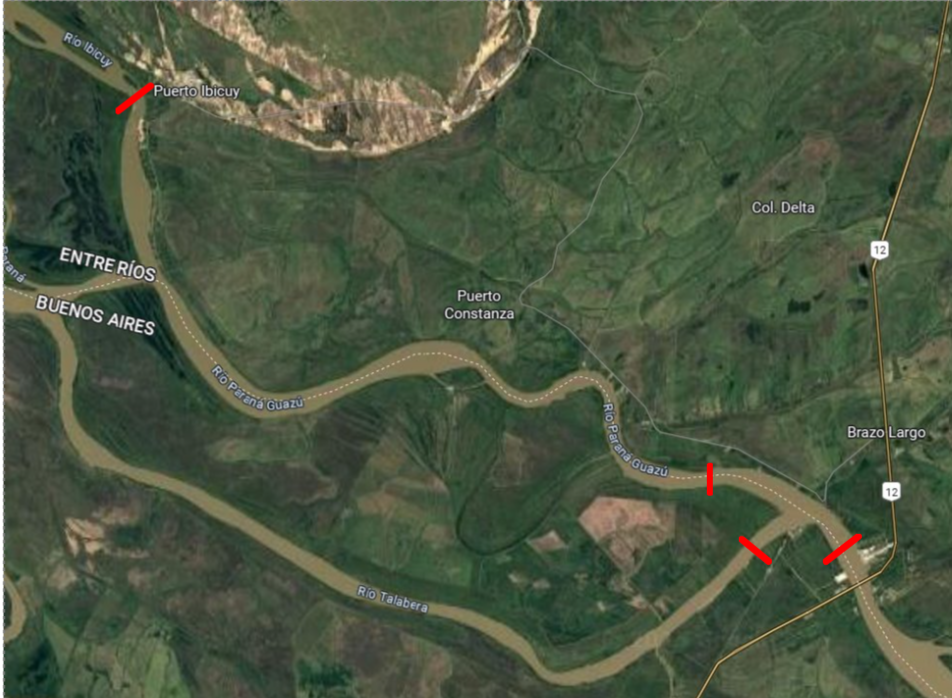
\includegraphics[width=0.5\linewidth]{figures/ch4/Critical measurement points.png}
    \caption{Critical Cross Section Measurements}
    \label{fig:fieldwork cross sections}
\end{figure}
During the field trip, one half of the group will work together with the INA team of employees who join us. The team consists of one skipper who will be responsible for driving of the boat and one supervisor who will help us with taking the measurements of the data.
The program of the two boat days will consist of going over the indicated critical cross sections (in red on Figure 4.2) a total of 4 times, using the equipment of INA to save the necessary information of the river.

\textit{Discharge}:

The first obtained data is the discharge 

\textit{Flow velocity}:

Furthermore, the group will also measure the flow velocity of the river at these given points.

\textit{Suspended sediment }:

Moving on, it is also in our interest to gather data on the suspended sediment of the river. This is done through 

\textit{Bed load}:

Lastly, the bed load is a necessary parameter for 

\section{Setting up the Sediment Balance}
Using the flow velocity we can derive the concentration of the sediment in the study area. This can be done for several locations in order to get an idea of the quantities of sediment that come in through the Rio Ibicuy, the Entre Rios and the Rio Talabera. Then the last critical point will help us determine the continuation of the concentration of the sediment in the Rio Parana so that any inconsistencies can be linked with the amount of extracted sand in the intersection of the Parana Guazu and Rio Talabera (in the middle of the three critical points on the right hand side of Figure 4.2).

A mathematical expression/derivation will be explained:
STEFANOOOOOOOOOOO

\section{Multidisciplinary approach}
The aim of this report is to present a comprehensive assessment of the sustainability of sand mining in the Paraná River. To capture the full scope of the issue, a multidisciplinary approach is adopted. Accordingly, the impacts of sand mining are examined from several perspectives, reflecting the expertise of the authors:

\begin{itemize}
    \item \textbf{Hydraulic}: assessment of the sediment balance and future river flow projections.
    \item \textbf{Geotechnical}: evaluation of risks to riverbank stability and identification of possible mitigation measures.
    \item \textbf{Structural}: analysis of potential effects on existing infrastructure, along with consideration of structural measures such as quay walls or stone revetments.
\end{itemize}